\chapter{El ojo y sus fotorreceptores}\label{ch:g11:the-eye}

En una noche sin luna, lejos de cualquier farola, ves el camino pero no
sus colores; la cazadora roja de un amigo es una forma gris. Mira de
frente a una estrella débil y desaparece; mira un poco de lado y
reaparece. Las dos rarezas vienen de la retina, la fina lámina del
fondo del \omterm{def:g11:the-eye:parts}{ojo} donde la luz se convierte en señal nerviosa: dos clases
de \omterm{def:g10:cells-common-unit:cell}{células} receptoras, repartidas de forma desigual, una de ellas ciega
al color y la otra ciega en la oscuridad. Este capítulo desmonta el \omterm{def:g11:the-eye:parts}{ojo}
desde la córnea hasta el nervio óptico, y lee, en los \omterm{def:g10:universal-dna:gene}{genes} de los
pigmentos de la retina, un fragmento de nuestra historia evolutiva.

\section{El ojo como instrumento óptico}

\begin{definition}[Las partes del ojo]\label{def:g11:the-eye:parts}
El \emph{ojo}\index{ojo} es un globo de unos \qty{24}{mm} de lado a
lado. La luz entra por la \emph{córnea} transparente, atraviesa la
\emph{pupila} --- la abertura del \emph{iris} coloreado, que se ensancha
en la oscuridad y se estrecha con luz fuerte --- y el
\emph{cristalino}, cruza la gelatina transparente del \emph{humor
vítreo} y llega a la \emph{retina}, la capa sensible a la luz que
tapiza el fondo del globo. La córnea y el cristalino forman juntos,
sobre la retina, una pequeña imagen invertida de la escena; el
cristalino, cuya curvatura pueden cambiar unos músculos, ajusta el
enfoque de los objetos lejanos a los cercanos (la
\emph{acomodación}). El \emph{nervio óptico} sale del fondo del ojo y
lleva al encéfalo las señales de la retina.
\end{definition}

\begin{omfigure}
\begin{tikzpicture}
  \node[anchor=south west, inner sep=0] (img) at (0,0)
    {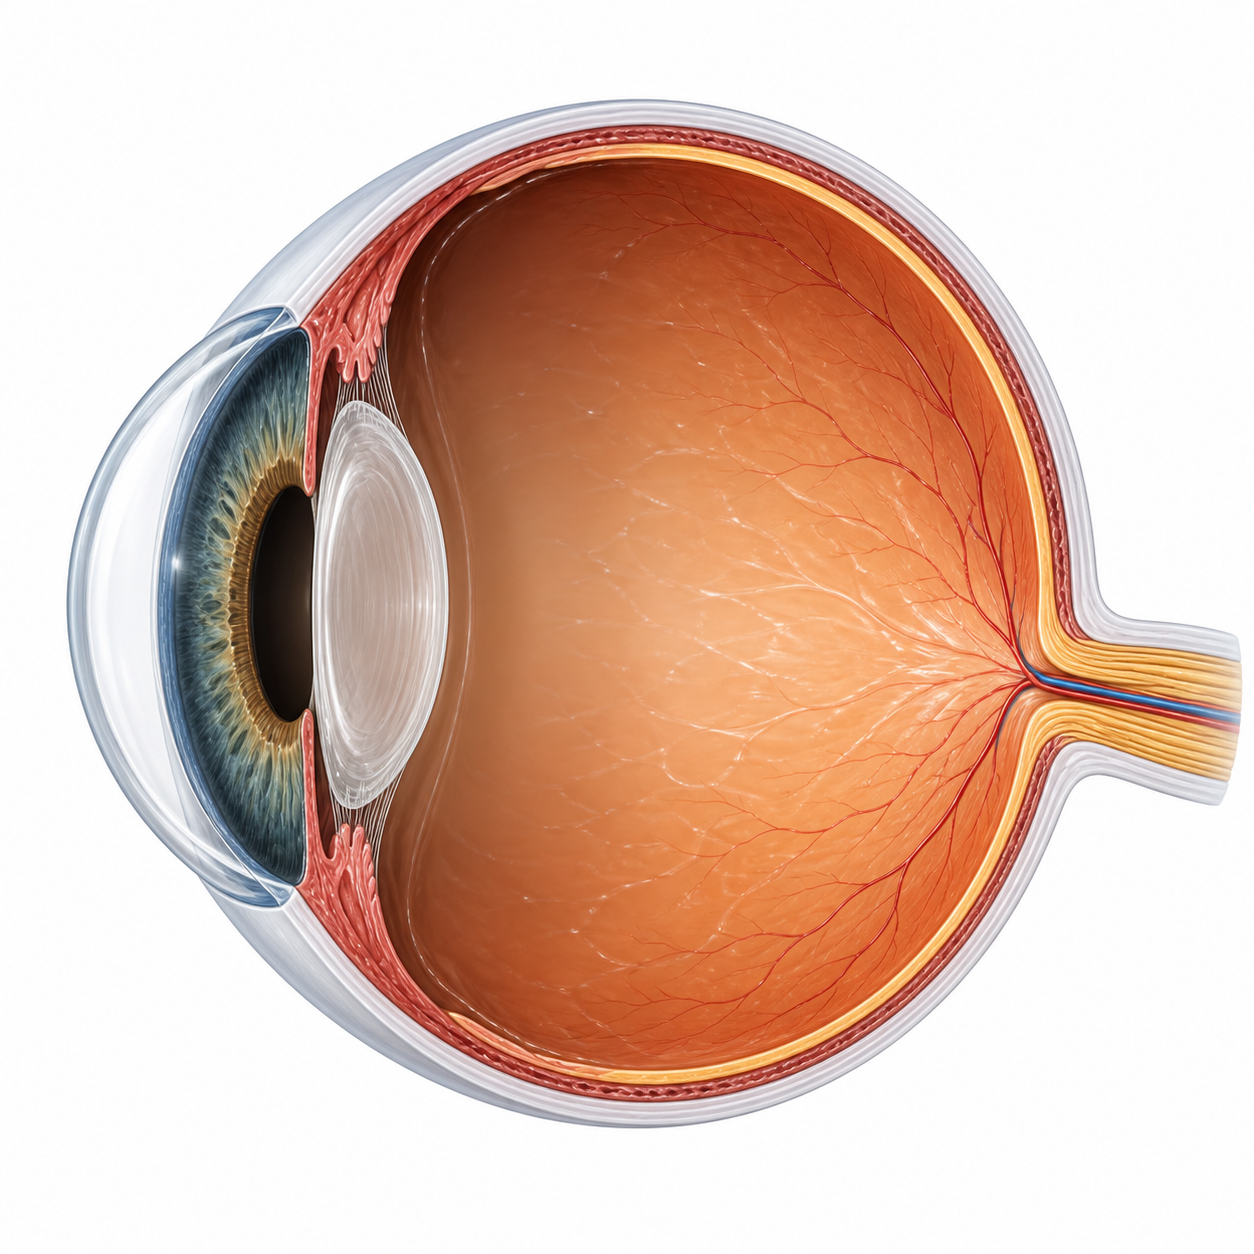
\includegraphics[width=0.46\linewidth]{images/book2/ai/fig-eye-cutaway.png}};
  \begin{scope}[x={(img.south east)}, y={(img.north west)},
      every node/.style={font=\small}]
    \draw[omDef, thick] (0.10,0.55) -- (-0.05,0.80) node[left] {córnea};
    \draw[omDef, thick] (0.18,0.36) -- (-0.05,0.20) node[left] {iris y pupila};
    \draw[omDef, thick] (0.26,0.50) -- (-0.05,0.50) node[left] {cristalino};
    \draw[omDef, thick] (0.55,0.50) -- (0.55,-0.06) node[below] {humor vítreo};
    \draw[omDef, thick] (0.83,0.76) -- (1.05,0.88) node[right] {retina};
    \draw[omDef, thick] (0.95,0.40) -- (1.05,0.20) node[right] {nervio óptico};
  \end{scope}
\end{tikzpicture}

{\small El \omterm{def:g11:the-eye:parts}{ojo} en corte horizontal. La córnea y el cristalino enfocan
la luz; la retina, al fondo, la convierte en señales que salen por el
nervio óptico.}
\end{omfigure}

\begin{example}[El enfoque y sus fallos]\label{ex:g11:the-eye:focus}
Un \omterm{def:g11:the-eye:parts}{ojo} relajado enfoca sobre la retina los objetos lejanos; para leer a
\qty{25}{cm}, el cristalino tiene que abombarse. Un \omterm{def:g11:the-eye:parts}{ojo} algo demasiado
largo enfoca los objetos lejanos por delante de la retina --- es la
miopía, que se corrige con una lente divergente; un \omterm{def:g11:the-eye:parts}{ojo} demasiado
corto, o un cristalino que se ha endurecido con la edad, no consigue
enfocar los objetos cercanos --- es la hipermetropía, que se corrige
con una lente convergente. En ambos casos la retina está intacta: el
fallo es óptico, y las gafas devuelven la imagen al sitio donde están
los receptores.
\end{example}

\section{La retina}

\begin{definition}[Fotorreceptores]\label{def:g11:the-eye:photoreceptors}
La retina contiene dos clases de \omterm{def:g10:cells-common-unit:cell}{células}
\emph{fotorreceptoras}\index{fotorreceptor}, llamadas así por su forma.
Los \emph{bastones}\index{bastón (retina)}, unos 120 millones,
responden a una luz muy tenue pero todos con el mismo pigmento: dan una
visión en tonos de gris por la noche. Los
\emph{conos}\index{cono (retina)}, unos 6 millones, necesitan más luz y
son de tres tipos, cada uno con un pigmento más sensible a una parte
distinta del espectro: dan la visión diurna y el color. Cada
fotorreceptor contiene un \emph{fotopigmento} --- una \omterm{def:g11:gene-expression:protein}{proteína}, una
\emph{opsina}\index{opsina}, que sostiene una pequeña molécula
absorbente de luz derivada de la vitamina A --- cuyo cambio de forma al
absorber un fotón pone en marcha la respuesta eléctrica de la \omterm{def:g10:cells-common-unit:cell}{célula}.
\end{definition}

\begin{omfigure}
\begin{tikzpicture}[font=\small, >=Stealth, line cap=round]
  % layers from front (left) to back (right); light comes from the left
  \draw[->, very thick, omProp] (-1.6,1.2) -- (-0.3,1.2) node[pos=0, above, omProp] {luz};
  % ganglion cells
  \foreach \y in {2.4,1.2,0.0} { \draw[thick, fill=omDef!25] (0.4,\y) circle (0.28); \draw[thick, omDef] (0.12,\y) -- (-0.6,\y) -- (-0.6,-1.4); }
  \node[anchor=north, align=center] at (0.4,-0.5) {células\\ ganglionares};
  \draw[->, thick, omDef] (-0.6,-1.4) -- (-0.6,-2.0) node[below, align=center] {hacia el\\ nervio óptico};
  % bipolar cells
  \foreach \y in {2.4,1.2,0.0} { \draw[thick, fill=omMeth!25] (2.2,\y) ellipse (0.22 and 0.36); \draw[thick] (0.68,\y) -- (1.98,\y); \draw[thick] (2.42,\y) -- (3.1,\y); }
  \node[anchor=north, align=center] at (2.2,-0.5) {células\\ bipolares};
  % photoreceptors: rods (tall rectangles) and cones (triangles)
  \foreach \y in {2.4,0.0} { \draw[thick, fill=gray!30] (3.1,\y-0.18) rectangle (5.0,\y+0.18); \node[font=\scriptsize] at (4.05,\y) {bastón}; }
  \draw[thick, fill=omThm!25] (3.1,1.2-0.22) -- (5.0,1.2-0.08) -- (5.0,1.2+0.08) -- (3.1,1.2+0.22) -- cycle;
  \node[font=\scriptsize] at (4.05,1.2) {cono};
  \node[anchor=north, align=center] at (4.5,-0.5) {fotorreceptores\\ (pigmento en la punta)};
  % pigment epithelium
  \fill[gray!60] (5.2,-0.2) rectangle (5.6,2.8);
  \node[anchor=west, align=left] at (5.7,1.2) {capa oscura\\ que absorbe\\ la luz dispersa};
  \node[anchor=south, align=center, font=\scriptsize] at (2.6,3.0) {la señal viaja de derecha a izquierda, contra la luz};
\end{tikzpicture}

{\small La retina, en corte. La luz atraviesa las capas transparentes
de \omterm{def:g10:cells-common-unit:cell}{células} nerviosas y llega a los \omterm{def:g11:the-eye:photoreceptors}{fotorreceptores} del fondo, cuyas
puntas absorbentes de luz miran al lado contrario; la señal viaja
después hacia delante, del receptor a la \omterm{def:g10:cells-common-unit:cell}{célula} bipolar y de esta a la
ganglionar, cuyas fibras forman el nervio óptico.}
\end{omfigure}

\begin{proposition}[Organización de la retina]\label{prop:g11:the-eye:organisation}
Los \omterm{def:g11:the-eye:photoreceptors}{fotorreceptores} están al fondo de la retina, contra una capa
oscura; la luz tiene que atravesar las demás capas para llegar a ellos.
Sus señales pasan a las \emph{\omterm{def:g10:cells-common-unit:cell}{células} bipolares} y después a las
\emph{\omterm{def:g10:cells-common-unit:cell}{células} ganglionares}, cuyas fibras largas --- alrededor de un
millón --- se agrupan en el nervio óptico. El reparto es desigual: en
la \emph{fóvea}, la pequeña depresión central hacia la que el \omterm{def:g11:the-eye:parts}{ojo}
apunta, solo hay \omterm{def:g11:the-eye:photoreceptors}{conos}, muy apretados y conectados cada uno a su propia
\omterm{def:g10:cells-common-unit:cell}{célula} ganglionar, lo que da la visión más nítida; lejos del centro
dominan los \omterm{def:g11:the-eye:photoreceptors}{bastones} y muchos de ellos comparten una \omterm{def:g10:cells-common-unit:cell}{célula}
ganglionar, lo que da sensibilidad a costa del detalle. Donde sale el
nervio óptico no hay ningún receptor: el \emph{punto ciego}.
\end{proposition}
\admitted

\begin{omfigure}
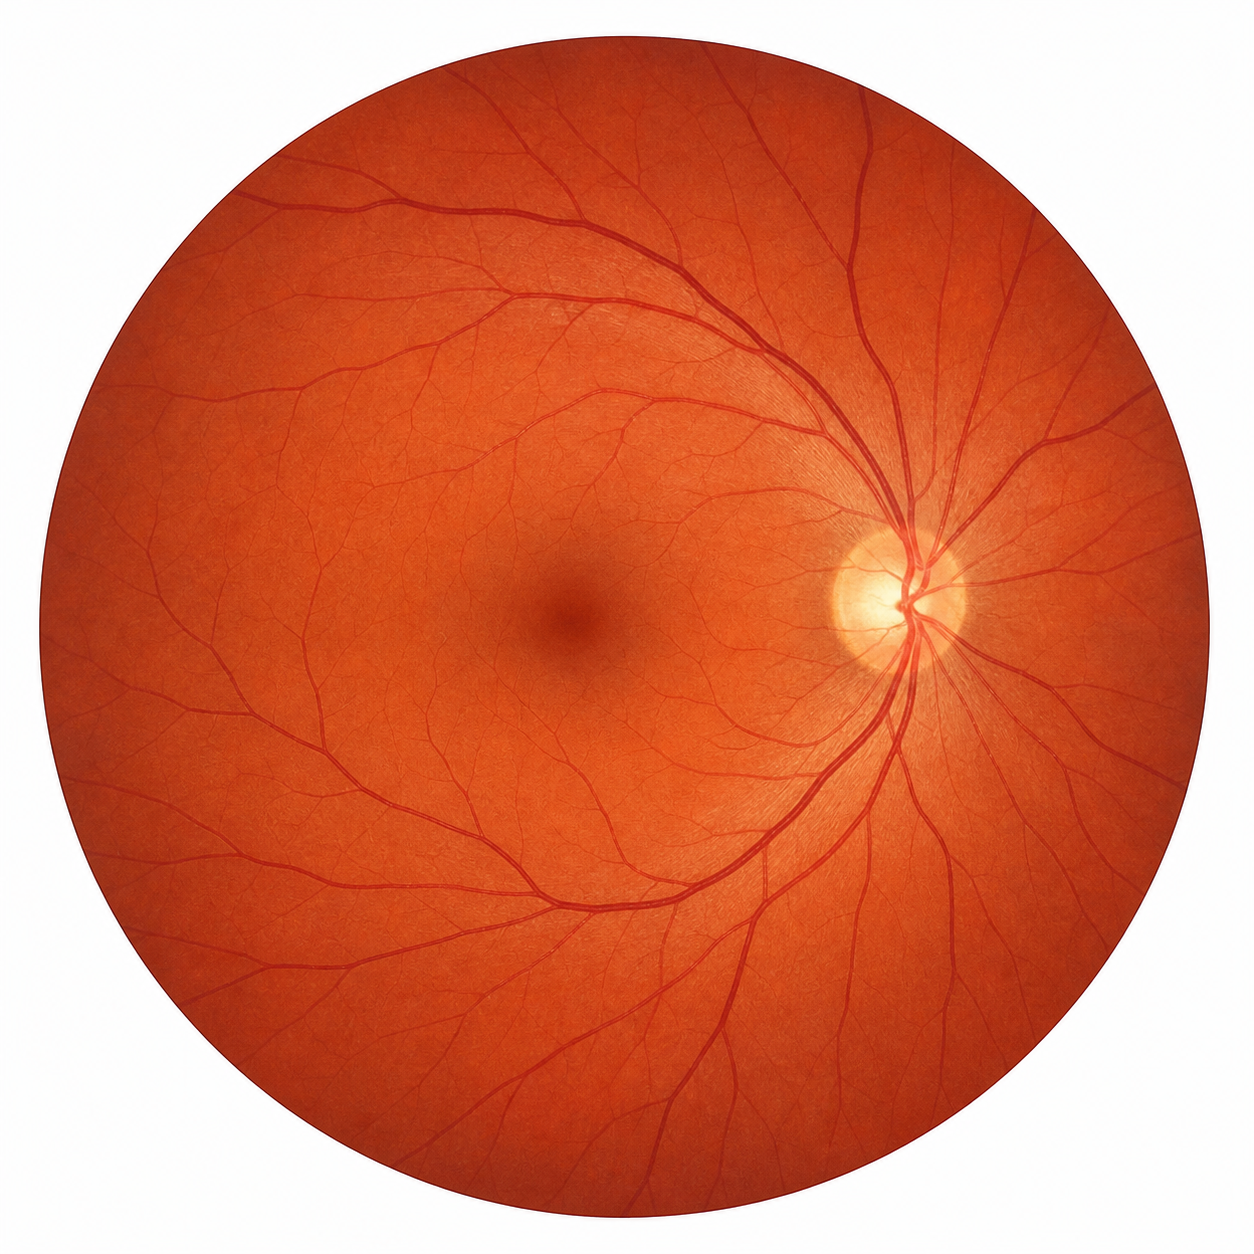
\includegraphics[width=0.42\linewidth]{images/book2/ai/g11-retina-fundus.png}

{\small La retina vista a través de la pupila con un oftalmoscopio: el
disco pálido por donde sale el nervio óptico y entran los vasos (el
punto ciego) y, más oscura y a un lado, la fóvea, donde los \omterm{def:g11:the-eye:photoreceptors}{conos} son
más densos.}
\end{omfigure}

\begin{example}[Las dos rarezas explicadas]\label{ex:g11:the-eye:oddities}
La estrella débil desaparece cuando se la mira de frente porque la
fóvea solo tiene \omterm{def:g11:the-eye:photoreceptors}{conos}, que necesitan más luz de la que da la estrella;
mirada de lado, su luz cae sobre los \omterm{def:g11:the-eye:photoreceptors}{bastones}, que la detectan. La
cazadora es gris de noche porque los \omterm{def:g11:the-eye:photoreceptors}{bastones} que la ven tienen un solo
pigmento: pueden informar de cuánta luz hay, no de qué longitud de
onda. El color es una comparación entre los tres tipos de \omterm{def:g11:the-eye:photoreceptors}{conos}, y los
\omterm{def:g11:the-eye:photoreceptors}{conos} callan en la oscuridad.
\end{example}

\section{El color: tres pigmentos}

\begin{proposition}[La visión del color]\label{prop:g11:the-eye:colour}
Cada tipo de cono contiene una de tres \omterm{def:g11:the-eye:photoreceptors}{opsinas}, con máximos de
absorción cercanos a \qty{420}{nm} (\omterm{def:g11:the-eye:photoreceptors}{conos} S, azul), \qty{530}{nm}
(\omterm{def:g11:the-eye:photoreceptors}{conos} M, verde) y \qty{560}{nm} (\omterm{def:g11:the-eye:photoreceptors}{conos} L, rojo). Una luz dada excita
los tres tipos en proporciones que dependen de su longitud de onda; el
encéfalo lee el color a partir de esas proporciones. Una persona a la
que le falta un tipo de cono confunde los colores que ese tipo
distinguía: sin \omterm{def:g11:the-eye:photoreceptors}{conos} L o M funcionales, el rojo y el verde son
difíciles de distinguir --- es el \emph{daltonismo para el rojo y el
verde}, que afecta a alrededor del 8\% de los hombres y al 0,5\% de las
mujeres.
\end{proposition}
\admitted

\begin{omfigure}
\begin{tikzpicture}
\begin{axis}[
  width=0.9\linewidth, height=5.8cm,
  axis x line=bottom, axis y line=left,
  xmin=380, xmax=700, ymin=0, ymax=110,
  xlabel={longitud de onda (nm)}, ylabel={absorción (\% del máximo)},
  xlabel style={font=\small, at={(axis description cs:0.5,-0.12)}, anchor=north},
  ylabel style={font=\small},
  tick label style={font=\small}, xtick={400,450,500,550,600,650,700}, ytick={0,50,100},
  legend style={at={(0.5,-0.3)}, anchor=north, legend columns=4, font=\small, draw=none},
]
\addplot[thick, omDef, smooth] coordinates {(380,40) (400,75) (420,100) (440,88) (460,55) (480,25) (500,8) (520,2) (540,0)};
\addplot[thick, gray, dashed, smooth] coordinates {(400,10) (430,35) (460,70) (480,90) (500,100) (520,90) (540,65) (560,38) (580,18) (600,7) (620,2) (640,0)};
\addplot[thick, omMeth, smooth] coordinates {(420,5) (450,20) (480,50) (510,85) (530,100) (550,90) (570,65) (590,38) (610,18) (630,7) (650,2) (670,0)};
\addplot[thick, omThm, smooth] coordinates {(440,5) (470,18) (500,40) (530,80) (560,100) (580,92) (600,70) (620,42) (640,20) (660,8) (680,3) (700,1)};
\legend{conos S (azul), bastones, conos M (verde), conos L (rojo)}
\end{axis}
\end{tikzpicture}

{\small Absorción de los cuatro fotopigmentos frente a la longitud de
onda. Cada una es ancha y se solapan; una luz amarilla de
\qty{580}{nm} excita mucho los \omterm{def:g11:the-eye:photoreceptors}{conos} L, moderadamente los M y nada los
S --- esa proporción es lo que significa ``amarillo'' para el
encéfalo.}
\end{omfigure}

\begin{example}[Leer las curvas]\label{ex:g11:the-eye:curves}
Luz de \qty{500}{nm}: \omterm{def:g11:the-eye:photoreceptors}{conos} S al 8\%, M al 75\%, L al 40\% --- se ve
azul verdoso. Luz de \qty{620}{nm}: S a 0, M al 10\%, L al 42\% ---
roja. Una persona sin \omterm{def:g11:the-eye:photoreceptors}{conos} L recibe, para las dos, solo un valor S y
uno M, y la segunda luz le da S~0, M~10: apenas distinguible de un
verde tenue. Los colores que habría separado el tipo que falta se
funden en uno.
\end{example}

\section{Los genes de las opsinas: una familia con historia}

\begin{proposition}[Genes de las opsinas]\label{prop:g11:the-eye:genes}
Cada \omterm{def:g11:the-eye:photoreceptors}{opsina} la codifica su propio \omterm{def:g10:universal-dna:gene}{gen}. El \omterm{def:g10:universal-dna:gene}{gen} de la \omterm{def:g11:the-eye:photoreceptors}{opsina} S está en un
\omterm{def:g11:cell-cycle-mitosis:chromosome}{cromosoma} corriente; los \omterm{def:g10:universal-dna:gene}{genes} de las \omterm{def:g11:the-eye:photoreceptors}{opsinas} M y L están uno al lado
del otro en el \omterm{def:g11:cell-cycle-mitosis:chromosome}{cromosoma} X. Las \omterm{def:g10:chemistry-of-life:families}{proteínas} L y M se diferencian en solo
15 de sus 364 \omterm{def:g10:chemistry-of-life:families}{aminoácidos} (un 96\% idénticas), y la \omterm{def:g11:gene-expression:protein}{proteína} S en más
de la mitad de sus posiciones respecto de cualquiera de las dos. Al
estar en el X, un \omterm{def:g10:universal-dna:gene}{alelo} M o L no funcional se expresa en todo varón que
lo lleve y solo en las mujeres que llevan dos --- el patrón del
\cref{ch:g11:genes-and-disease}, y la razón de que el daltonismo para
el rojo y el verde sea dieciséis veces más frecuente en los hombres.
\end{proposition}
\admitted

\begin{proposition}[Una familia de genes nacida de duplicaciones]\label{prop:g11:the-eye:family}
Los tres \omterm{def:g10:universal-dna:gene}{genes} de las \omterm{def:g11:the-eye:photoreceptors}{opsinas}, y el del pigmento de los \omterm{def:g11:the-eye:photoreceptors}{bastones}, son
versiones de un mismo \omterm{def:g10:universal-dna:gene}{gen} ancestral copiado por \emph{duplicación} y
divergido después por \omterm{def:g11:mutations:mutation}{mutación}. Sus grados de parecido datan las
copias: las líneas S y L/M se separaron muy pronto en la historia de
los \omterm{def:g10:common-ancestry:bodyplan}{vertebrados}, hace unos 500 millones de años; los \omterm{def:g10:universal-dna:gene}{genes} L y M
surgieron de una duplicación hace unos 30 o 40 millones de años en el
antepasado de los primates del Viejo Mundo, cuyos descendientes ---
monos, simios y humanos --- tienen tres tipos de \omterm{def:g11:the-eye:photoreceptors}{conos}, mientras que
casi todos los demás mamíferos tienen dos.
\end{proposition}
\begin{proof}[Pruebas experimentales]
La comparación de secuencias: los \omterm{def:g10:universal-dna:gene}{genes} L y M son idénticos en un 96\%
y contiguos en el X --- la firma de una duplicación en tándem reciente;
cada uno es idéntico en un 43\% aproximadamente al \omterm{def:g10:universal-dna:gene}{gen} S, y los tres en
torno a un 40\% al \omterm{def:g10:universal-dna:gene}{gen} de la \omterm{def:g11:the-eye:photoreceptors}{opsina} de los \omterm{def:g11:the-eye:photoreceptors}{bastones}, las copias más
lejanas. Los perros, el ganado vacuno y casi todos los mamíferos tienen
un solo \omterm{def:g10:universal-dna:gene}{gen} de \omterm{def:g11:the-eye:photoreceptors}{opsina} ligado al X, en la posición donde los primates
tienen dos; los monos del Nuevo Mundo tienen uno, con varios \omterm{def:g10:universal-dna:gene}{alelos}, y
solo las hembras que llevan dos \omterm{def:g10:universal-dna:gene}{alelos} distintos ven tres colores. El
número de \omterm{def:g10:universal-dna:gene}{genes} coincide con el número de \omterm{def:g11:the-eye:photoreceptors}{conos} en cada linaje, y el
árbol de los \omterm{def:g10:universal-dna:gene}{genes} coincide con el árbol de las \omterm{def:g10:biodiversity-scales:species}{especies}.
\end{proof}

\begin{omfigure}
\begin{tikzpicture}[font=\small, line cap=round]
  % gene tree: root -> (rod opsin) ; (S) ; (L/M split)
  \draw[thick] (0,2) -- (1.5,2);
  \draw[thick] (1.5,2) -- (1.5,3.4) -- (9,3.4);
  \draw[thick] (1.5,2) -- (1.5,0.6) -- (3.2,0.6);
  \draw[thick] (3.2,0.6) -- (3.2,1.8) -- (9,1.8);
  \draw[thick] (3.2,0.6) -- (3.2,-0.6) -- (7.6,-0.6);
  \draw[thick] (7.6,-0.6) -- (7.6,0.2) -- (9,0.2);
  \draw[thick] (7.6,-0.6) -- (7.6,-1.4) -- (9,-1.4);
  \fill[omThm] (1.5,2) circle (2.5pt); \fill[omThm] (3.2,0.6) circle (2.5pt); \fill[omThm] (7.6,-0.6) circle (2.5pt);
  \node[anchor=west] at (9.1,3.4) {rodopsina (bastones)};
  \node[anchor=west] at (9.1,1.8) {opsina S (conos azules)};
  \node[anchor=west] at (9.1,0.2) {opsina M (conos verdes)};
  \node[anchor=west] at (9.1,-1.4) {opsina L (conos rojos)};
  \node[anchor=south, font=\scriptsize, omThm] at (1.5,3.5) {duplicación, muy temprana};
  \node[anchor=north, font=\scriptsize, omThm, align=center] at (3.2,-0.75) {duplicación\\ hace $\sim$500 millones de años};
  \node[anchor=north, font=\scriptsize, omThm, align=center] at (7.6,-1.55) {duplicación\\ hace $\sim$35 millones de años};
  \node[anchor=east] at (-0.1,2) {gen ancestral};
  \draw[->, gray] (0,-2.3) -- (9,-2.3) node[midway, below, font=\scriptsize] {tiempo};
\end{tikzpicture}

{\small La familia de \omterm{def:g10:universal-dna:gene}{genes} de las \omterm{def:g11:the-eye:photoreceptors}{opsinas}. Cada punto rojo es una
duplicación: un \omterm{def:g10:universal-dna:gene}{gen} se convirtió en dos, y las copias divergieron
después por \omterm{def:g11:mutations:mutation}{mutación}. La más reciente, la de L/M, solo se encuentra en
los primates del Viejo Mundo y les dio un tercer cono.}
\end{omfigure}

\begin{example}[Lo que cambió una duplicación]\label{ex:g11:the-eye:duplication}
Un mono con dos tipos de \omterm{def:g11:the-eye:photoreceptors}{conos} ve el bosque en dos dimensiones de
color, y la fruta madura es difícil de distinguir entre el follaje.
Tras la duplicación L/M, una copia pudo mutar hacia longitudes de onda
más largas mientras la otra conservaba la original --- un tercer cono, y
el rojo maduro contra el verde. La \omterm{def:g11:mutations:mutation}{mutación} que más tarde estropea una
copia en el 8\% de los hombres simplemente devuelve el \omterm{def:g11:the-eye:parts}{ojo} al estado
ancestral de dos \omterm{def:g11:the-eye:photoreceptors}{conos}.
\end{example}

\begin{method}[Razonar sobre un caso de visión del color]\label{met:g11:the-eye:case}
\begin{enumerate}
  \item ¿Qué tipo de cono falta o está alterado? Léelo en los colores
        que se confunden (rojo y verde: L o M; azul y amarillo, raro:
        S).
  \item ¿Qué \omterm{def:g10:universal-dna:gene}{gen}, y en qué \omterm{def:g11:cell-cycle-mitosis:chromosome}{cromosoma}? L y M en el X, y S en otro.
  \item Aplica la herencia: \omterm{def:g11:genes-and-disease:genetic}{recesiva} ligada al X para el rojo y el
        verde --- los hijos varones de madres \omterm{def:g11:genes-and-disease:genetic}{portadoras} afectados una
        vez de cada dos, y las hijas de padres afectados todas
        \omterm{def:g11:genes-and-disease:genetic}{portadoras}.
  \item Relaciónalo con la familia de \omterm{def:g10:universal-dna:gene}{genes}: una copia perdida, o unas
        copias L y M hechas demasiado parecidas por un intercambio
        entre los \omterm{def:g10:universal-dna:gene}{genes} contiguos.
\end{enumerate}
\end{method}

\begin{remark}[Del ojo al encéfalo]\label{rem:g11:the-eye:tobrain}
La retina no ve; convierte y empieza a clasificar. El millón de fibras
del nervio óptico lleva una descripción codificada --- contrastes,
bordes, proporciones de las respuestas de los \omterm{def:g11:the-eye:photoreceptors}{conos} --- hasta el
encéfalo, donde la recoge el capítulo siguiente. Lo que llamamos ver
ocurre allí, construido sobre las señales de las \omterm{def:g10:cells-common-unit:cell}{células} descritas aquí
y sobre nada más: una persona cuyas retinas funcionan pero cuyo
encéfalo visual está dañado es ciega, y otra cuyo encéfalo visual
funciona pero cuyos \omterm{def:g11:the-eye:photoreceptors}{fotorreceptores} han muerto también lo es.
\end{remark}

\section{Ejercicios}

\begin{exercise}[$\star$]\label{exo:g11:the-eye:1}
Enumera, en orden, las estructuras que atraviesa la luz desde el
exterior hasta los \omterm{def:g11:the-eye:photoreceptors}{fotorreceptores}.
\end{exercise}

\begin{exercise}[$\star$]\label{exo:g11:the-eye:2}
Compara los \omterm{def:g11:the-eye:photoreceptors}{bastones} y los \omterm{def:g11:the-eye:photoreceptors}{conos}: número, sensibilidad, pigmentos y
clase de visión.
\end{exercise}

\begin{exercise}[$\star$]\label{exo:g11:the-eye:3}
¿Qué son la fóvea y el punto ciego?
\end{exercise}

\begin{exercise}[$\star$]\label{exo:g11:the-eye:4}
En la figura de la absorción, ¿qué pigmentos absorben la luz de
\qty{450}{nm}, y con qué intensidad?
\end{exercise}

\begin{exercise}[$\star$]\label{exo:g11:the-eye:5}
¿En qué \omterm{def:g11:cell-cycle-mitosis:chromosome}{cromosoma} están los \omterm{def:g10:universal-dna:gene}{genes} de las \omterm{def:g11:the-eye:photoreceptors}{opsinas} L y M, y qué se sigue
para la herencia del daltonismo para el rojo y el verde?
\end{exercise}

\begin{exercise}[$\star\star$]\label{exo:g11:the-eye:6}
Explica por qué no vemos colores de noche y por qué una estrella débil
se ve mejor de lado.
\end{exercise}

\begin{exercise}[$\star\star$]\label{exo:g11:the-eye:7}
Dos luces excitan los \omterm{def:g11:the-eye:photoreceptors}{conos} así: luz 1, S 0, M 60, L 100; luz 2, S 0,
M 30, L 50. ¿Son del mismo color? ¿Del mismo brillo? Explícalo.
\end{exercise}

\begin{exercise}[$\star\star$]\label{exo:g11:the-eye:8}
Un hombre daltónico se casa con una mujer sin familiares daltónicos.
Da la visión del color de sus hijos varones, de sus hijas y de los
hijos varones de sus hijas.
\end{exercise}

\begin{exercise}[$\star\star$]\label{exo:g11:the-eye:9}
¿Por qué el daltonismo para el rojo y el verde es dieciséis veces más
frecuente en los hombres que en las mujeres? Calcula la frecuencia
esperada en las mujeres a partir del 8\% de los hombres.
\end{exercise}

\begin{exercise}[$\star\star$]\label{exo:g11:the-eye:10}
Los \omterm{def:g10:universal-dna:gene}{genes} L y M son idénticos en un 96\%, y cada uno lo es en un 43\%
al S. Explica cómo esas dos cifras datan una duplicación respecto de la
otra.
\end{exercise}

\begin{exercise}[$\star\star$]\label{exo:g11:the-eye:11}
Casi todos los mamíferos tienen dos tipos de \omterm{def:g11:the-eye:photoreceptors}{conos}, y los primates del
Viejo Mundo tres. Explica la diferencia con una duplicación y di por
qué pudo conservarse.
\end{exercise}

\begin{exercise}[$\star\star\star$]\label{exo:g11:the-eye:12}
A una persona le faltan los \omterm{def:g11:the-eye:photoreceptors}{conos} S. ¿Qué colores confunde? Explica por
qué esa condición es rara y por qué es igual de frecuente en ambos
sexos.
\end{exercise}

\begin{exercise}[$\star\star\star$]\label{exo:g11:the-eye:13}
Los \omterm{def:g11:the-eye:photoreceptors}{conos} de la fóvea están separados \qty{2.5}{\micro m} y la
distancia focal del \omterm{def:g11:the-eye:parts}{ojo} es de unos \qty{17}{mm}. Calcula el ángulo más
pequeño que pueden subtender dos puntos y caer aún sobre \omterm{def:g11:the-eye:photoreceptors}{conos}
distintos, y el tamaño del detalle más pequeño que puede resolverse a
\qty{10}{m}. (Usa la aproximación de ángulos pequeños: ángulo en
radianes $=$ tamaño $/$ distancia.)
\end{exercise}

\begin{exercise}[$\star\star\star$]\label{exo:g11:the-eye:14}
En los monos del Nuevo Mundo, el único \omterm{def:g10:universal-dna:gene}{gen} de \omterm{def:g11:the-eye:photoreceptors}{opsina} ligado al X tiene
varios \omterm{def:g10:universal-dna:gene}{alelos} con distintas longitudes de onda máximas. Explica por qué
solo algunas hembras de esas \omterm{def:g10:biodiversity-scales:species}{especies} ven tres colores, y ningún macho.
\end{exercise}

\begin{exercise}[$\star\star\star$]\label{exo:g11:the-eye:15}
Una enfermedad destruye los \omterm{def:g11:the-eye:photoreceptors}{fotorreceptores} pero respeta el resto de la
retina. Explica por qué un implante que estimule eléctricamente las
\omterm{def:g10:cells-common-unit:cell}{células} ganglionares puede devolver algo de visión, y qué limita su
calidad.
\end{exercise}

\section{Problema: Tres pigmentos y una duplicación}

\begin{problem}[{Problema de fin de semana --- la visión del color
desmontada: las respuestas de los conos a un espectro, una familia con
daltonismo, los genes de las opsinas comparados y la nitidez que puede
alcanzar una fóvea}]
\label{pb:g11:the-eye:1}
Usa la figura de la absorción. Una prueba presenta luces de
\qty{470}{nm}, \qty{530}{nm}, \qty{590}{nm} y \qty{650}{nm}.

\medskip
\noindent\textbf{Parte I --- Los \omterm{def:g11:the-eye:photoreceptors}{conos} responden.}
\begin{enumerate}
  \item Para cada luz, lee la respuesta aproximada de los \omterm{def:g11:the-eye:photoreceptors}{conos} S, M y
        L.
  \item ¿Qué luz excita los tres tipos? ¿Cuál excita solo a uno?
  \item Una persona sin \omterm{def:g11:the-eye:photoreceptors}{conos} L recibe solo los valores S y M. ¿Cuáles
        dos de las cuatro luces le resultan difíciles de distinguir?
        Justifícalo con los números.
  \item Una persona sin \omterm{def:g11:the-eye:photoreceptors}{conos} M: ¿qué pareja confunde?
  \item Explica por qué ninguna de las dos personas es ``ciega al
        rojo'', pero las dos distinguen mal el rojo del verde.
\end{enumerate}

\medskip
\noindent\textbf{Parte II --- Una familia.}
Nora ve los colores con normalidad; su padre es daltónico para el rojo
y el verde. Se casa con Sam, que ve con normalidad.
\begin{enumerate}[resume]
  \item Da el \omterm{def:g11:enzymes-and-phenotype:phenotype}{genotipo} de Nora para el \omterm{def:g10:universal-dna:gene}{gen} de \omterm{def:g11:the-eye:photoreceptors}{opsina} ligado al X y
        justifícalo.
  \item Da los \omterm{def:g11:enzymes-and-phenotype:phenotype}{genotipos} y la visión del color de sus posibles hijos
        varones e hijas, con probabilidades.
  \item Su hija Inés, con visión del color normal, se casa con un
        hombre daltónico. Calcula la probabilidad de que Inés sea
        \omterm{def:g11:genes-and-disease:genetic}{portadora} y después la probabilidad de que una hija suya sea
        daltónica.
  \item Explica por qué una hija daltónica tiene siempre un padre
        daltónico.
  \item La madre del padre de Nora veía los colores con normalidad.
        ¿Era necesariamente \omterm{def:g11:genes-and-disease:genetic}{portadora}? Explícalo.
\end{enumerate}

\medskip
\noindent\textbf{Parte III --- Los \omterm{def:g10:universal-dna:gene}{genes}.}
Identidades entre las secuencias proteicas de las \omterm{def:g11:the-eye:photoreceptors}{opsinas}: L--M 96\%,
L--S 43\%, M--S 43\%, S--rodopsina 41\%.
\begin{enumerate}[resume]
  \item Dibuja, o describe, el árbol de los cuatro \omterm{def:g10:universal-dna:gene}{genes} que implican
        estas cifras.
  \item Si las diferencias se acumulan a ritmo constante y la
        duplicación L/M tiene 35 millones de años, estima la
        antigüedad de la separación entre S y L/M.
  \item Los \omterm{def:g10:universal-dna:gene}{genes} L y M están uno al lado del otro en el X. Explica
        cómo un intercambio desigual entre ellos durante la meiosis
        puede producir un X que solo lleve uno de los dos, y qué
        visión del color resulta.
  \item Esos intercambios son la causa más frecuente del daltonismo
        para el rojo y el verde. ¿Por qué dos \omterm{def:g10:universal-dna:gene}{genes} contiguos y casi
        idénticos son especialmente propensos a ellos?
  \item La duplicación L/M se encuentra en todos los primates del Viejo
        Mundo y en ningún otro mamífero. ¿Qué dice eso sobre cuándo y
        en quién ocurrió?
\end{enumerate}

\medskip
\noindent\textbf{Parte IV --- La nitidez de la fóvea.}
Los \omterm{def:g11:the-eye:photoreceptors}{conos} de la fóvea están separados \qty{2.5}{\micro m}; la distancia
focal del \omterm{def:g11:the-eye:parts}{ojo} es de \qty{17}{mm}. Usa ángulo (radianes) $=$ tamaño $/$
distancia.
\begin{enumerate}[resume]
  \item Calcula el ángulo que subtienden dos \omterm{def:g11:the-eye:photoreceptors}{conos} vecinos, en radianes
        y en minutos de arco ($1' = \num{2.9e-4}$ rad).
  \item ¿Cuál es el detalle de letra más pequeño resoluble a
        \qty{6}{m}? Compáralo con los trazos de las letras de una tabla
        optométrica, de unos \qty{1.7}{mm} a esa distancia para una
        visión ``normal''.
  \item Lejos de la fóvea, 100 \omterm{def:g11:the-eye:photoreceptors}{bastones} comparten una \omterm{def:g10:cells-common-unit:cell}{célula}
        ganglionar. Estima el ángulo resoluble allí y explica qué se
        gana a cambio.
  \item Los \omterm{def:g11:the-eye:photoreceptors}{conos} de la fóvea de un águila están el doble de apretados
        y su \omterm{def:g11:the-eye:parts}{ojo} es algo mayor. ¿Por qué factor es más fina su
        \omterm{def:g10:cells-common-unit:magnification}{resolución}?
  \item Enuncia el resultado: los tres tipos de \omterm{def:g11:the-eye:photoreceptors}{conos} y la luz a la que
        cada uno es ciego, el único suceso genético que dio a los
        primates el tercero y el ángulo que resuelve la fóvea.
\end{enumerate}
\end{problem}
